\documentclass{article}
\usepackage{blindtext}
\usepackage{titlesec}
\usepackage[utf8]{inputenc}
\usepackage[english, ukrainian]{babel}
\usepackage{amsmath, amssymb}
\usepackage{mathrsfs}
\usepackage{tikz}
\usepackage[top = 1 cm, left = 2 cm, right = 1 cm, bottom = 2 cm]{geometry} 
\ifx\pdfoutput\undefined
\else
\usepackage[dvips]{graphicx}
\fi
\usepackage{graphicx}
\usepackage{amsthm}
\theoremstyle{definition}
\newtheorem{theorem}{\textcolor{Black}{Теорема}}[section]
\newtheorem{definition}{\textcolor{Black}{Визначення}}[section]


\newcommand{\NN}{\mathbb{N}} 
\newcommand{\ZZ}{\mathbb{Z}}
\newcommand{\QQ}{\mathbb{Q}}
\newcommand{\RR}{\mathbb{R}}
\newcommand{\CC}{\mathbb{C}}

\newcommand{\Max}{\displaystyle\max\limits}
\newcommand{\Min}{\displaystyle\min\limits}
\newcommand{\Sum}{\displaystyle\sum\limits}
\newcommand{\Int}{\displaystyle\int\limits}
\newcommand{\Lim}{\displaystyle\lim\limits}
\newcommand{\Prod}{\displaystyle\prod\limits}


\allowdisplaybreaks

\setlength{\parindent}{0pt}





\date{}

\usepackage[dvipsnames]{xcolor}
\usepackage{colortbl}
\usepackage[dvips]{graphicx}
\graphicspath{{noiseimages/}}
\usepackage[utf8]{inputenc}
\usepackage{wrapfig}
\usepackage{subcaption}
\usepackage[normalem]{ulem} 

\usepackage[utf8]{inputenc}
\usepackage[english, ukrainian, russian]{babel}
\title {\textbf{Зачем люди учат математический анализ?}}
\author{}

\begin{document}

\maketitle
\vspace{-50}
\begin{center}
 \small{\textit{для тех, кто отчаялся в его изучении после неудачных попыток сдать экзамен}}   
\end{center}
\begin{center}
 \small{\textit{и}}   
\end{center}
\begin{center}
 \small{\textit{для тех, кто хочет заработать миллион}}   
\end{center}
\vspace{45}

\setlength{\epigraphwidth}{0.4\textwidth}
\epigraph{«Вот представьте, что вы уснули на 500 лет, а потом проснулись. О чём бы вы спросили в первую очередь после своего пробуждения?» Гильберт ответил: «Я бы спросил, доказана ли гипотеза Римана»}{}


\hspace{20}Уверена, сегодня вы точно открывали конспект по матанализу. У нас на примате это на завтрак, обед и ужин. Многие из нас задаются вопросом: "А зачем все это надо? Ладно там, построение функций и подсчёт объёма приплюснутого шара. Но если взять ряды, гамма-функции...\textbf{ О Боже!}" $\;$Каждый раз, штудируя теорию на очередной модуль, мы призадумываемся о том, что на самом деле все эти теоремы уже давно никто не использует. Попробую доказать, что это не так! Следующие 7 страниц - вовсе не обычный экскурс в историю математики и криптографии, и даже не очередная лекция по матанализу. Я пошагово продемонстрирую связь между нашей жизнью и теоремами, которые мы так любим учить:) 

\section{Ключ, сундук и австралийский друг}

\hspace{20}На самом деле матанализ сплошь и рядом! Каждую минуту мы используем его, когда отправляем сообщения с нашего телефона. Но обо всем по порядку:)




\hspace{20}Много кому придёт в голову идея отправить кому-то сообщение, чтобы прочитать его мог только тот, кому оно адресовано. В 21-ом веке информационные сигналы подобны \textbf{голубиной почте}: их легко перехватить. Разумеется, хотелось бы, чтобы те, кто перехватил информацию, по крайней мере не смогли ее прочесть. Отсюда возникает мораль, что свои данные нужно как-то зашифровать. Если говорить вкратце, зашифровать - значит физически что-то сделать с информацией, что-то заменить, где-то сместить. В конце получится какая-то бессмыслица, которую потом можно будет расшифровать. Если знать принцип шифрования, то потом становится легко прочесть нужную информацию. Между шифровальщиками и дешифровальщиками разразилась война, на протяжении 1000 лет соревнуются лучшие умы: одни пытаются зашифровать так, чтобы другие расшифровали, другие пытаются расшифровать то, что другие зашифровали. 
Объясню на примере алфавита и шифре \textbf{простой замены}, где каждый символ заменяется на другой символ произвольно. Например, А $\rightarrow$ Д, Б $\rightarrow$ Е и т.д. 
\begin{center}
    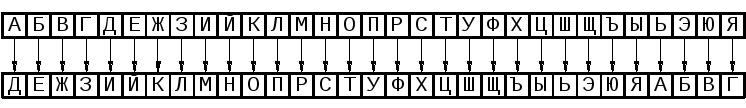
\includegraphics[width=0.8\linewidth]{alphabet.png}}
\end{center}
\newline \hspace{20}Сколько в этом случае вариантов? Комбинаторика подсказывает, что 32! (и это, друзья, не знак восклицания, а факториал). И это много! Если ручками попытаться перебрать все эти варианты, \textbf{может и жизни не хватить}. Если ваш назойливый младший брат перехватит ваше сообщение, записанное циклом простой замены, то ближайшие 10 лет он вас точно не потревожит, так как будет занят расшифровкой. Но очевидно, что и этот шифр легко взломать методом частотного анализа, прикинув, какие буквы чаще всего встречаются и какие слова из них можно составить. 
Люди - умный народ, поэтому смогли придумать алгоритм шифрования, который очень сложно взломать, а именно \textbf{RSA} (криптографический алгоритм с открытым ключом). Он-то как раз был основан на чистой математике. 




\hspace{20} Насколько быстро мы можем разложить число на два простых множителя? При малых числах, очевидно, быстро. А теперь представьте себе, что числа тысячезначные! В этом случае разложить на множители за разумное время не сможет даже суперкомпьютер. Отсюда мораль: если я знаю, как разложить число на множители, то я могу использовать это разложение, а никто другой - нет. И вот это как раз положено в \textbf{принцип шифрования}. Конечно же, эти самые числа не придумывают люди: их генерирует компьютер. 

\newline \hspace{20}
\begin{wrapfigure}{l}{0.4\textwidth}
 \vspace{-25pt}
  \begin{center}
    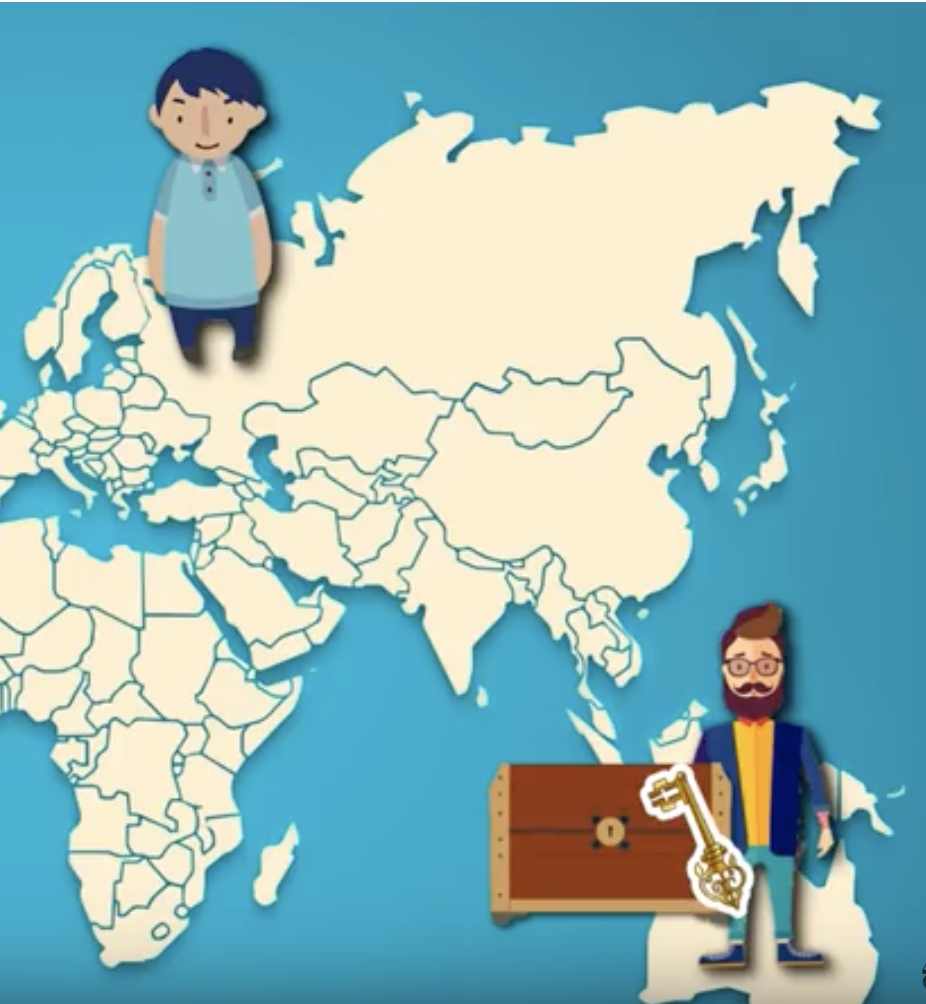
\includegraphics[width=0.4\textwidth]{australia.png}
  \end{center}
   \vspace{-20pt}
\end{wrapfigure}
Допустим, у меня есть \textbf{друг из Австралии}, который хочет получить от меня сообщение (сундук, для наглядности).
Чтобы его расшифровать, мне нужен ключ. Просто передать по почте его нельзя, так как его могут перехватить. Поэтому используется следующий алгоритм: мой друг САМ делает сундук, и САМ хранит у себя ключ (у меня ключа нет). Он отсылает мне ОТКРЫТЫЙ сундук, я в него кладу письмо и захлопываю его. Теперь я сама открыть сундук не могу, но и НИКТО другой не может! Дальше я отправляю этот сундук обратно, и мой друг откроет его СВОИМ ключом. 
То есть открыто по сети отправляется большое-большое число, равное произведению двух ПРОСТЫХ чисел, - это наш с вами сундук. А ключ от него (два исходных простых числа) хранится у меня, поэтому, расшифровать, если что, могу только я.\textbf{ И это довольно круто!}\\


\hspace{20}В общем, алгоритм шифрования RSA основан на том, что легко взять два (очень больших) простых числа и умножить их, в то время как очень трудно сделать обратное: взять очень большое число, учитывая, что у него есть только два простых фактора, и найти их. Как раз поэтому простые числа активно изучаются. На данный момент никто не знает быстрого алгоритма, чтобы разделить целое на его простые множители. А что если мы сможем знать распределения простых чисел, тем самым находить эти самые множители за считанные секунды? Тогда человек, нашедший своего рода формулу простых чисел, может \textbf{уничтожить все достижения современной криптографии} и продвинуть её на абсолютно новый уровень.

\newline \hspace{20}
\begin{wrapfigure}{r}{0.3\textwidth}
 \vspace{-50pt}
  \begin{center}
    
\includegraphics[width=0.3\textwidth]{emoji.png}
  \end{center}
   \vspace{-90pt}
\end{wrapfigure}

\section{Я вижу, но не могу поверить}

\newline \hspace{20} Говорят, что самый сложный способ заработать миллион долларов - доказать гипотезу Римана, которая, кстати говоря, входит в список семи задач тысячелетия. Какая ещё гипотеза, спросите вы? Мы ведь только что разговаривали о криптографии? А Риман к ней уж точно прямого отношения не имеет. Дочитайте до конца и обо всем узнаете:)
\newpage



\newline \hspace{20}



\newline \hspace{20}Эта гипотеза вроде как уже доказана математиком Майклом Фрэнсисом Атья, на заметку, одним из самых уважаемых и известных математиков современности! Давайте разберемся, что же он доказал или, возможно, не доказал?
Формулировка гипотезы звучит так:\\
\centerline{\textbf{\textit{действительная часть всех нетривиальных нулей дзета-функции равна $\dfrac{1}{2}$}}.} 

\hspace{20}Для многих это звучит как «абракадабра», так что \textbf{давайте разбираться}. Начнём издалека. С простых чисел. Как уже говорилось, в криптографии простые числа применяются сплошь и рядом. И одна из задач - понимать, как устроены простые числа, то есть как часто они встречаются, какое следующее простое число, насколько близко оно от предыдущего и т.д. Уже давно доказано, что их бесконечно много, но до сих пор мир тревожит вопрос о том, по какому принципу распределены простые числа по натуральному ряду. И существует ли точный \textbf{закон нахождения} этих \textbf{простых чисел}? Чтобы хоть как-то приблизиться к ответу на этот вопрос математиками была придумана функция распределения простых чисел. Для того, чтобы понять, что это такое, рассмотрим числовую последовательность. Сначала рассмотрим все натуральные числа от 1 до 10: среди них есть четыре простых числа:\\
\textit{1 $-$ 10: 2, 3, 5, 7 $\rightarrow$ 4}\\
Теперь рассмотрим все натуральные числа от 1 до 100, и мы увидим 25 простых чисел:\\
\textit{1 $-$ 100: 11, 13,...,89, 97 $\rightarrow$ 25}\\
И так далее:\\
\textit{1-1000: 101, 103,..., 991, 997 $\rightarrow$ 168}\\
\textit{1-10000: 1009, 1013,..., 9967, 9973 $\rightarrow$ 1229}\\
....
\newline \hspace{20}
\begin{wrapfigure}{r}{0.55\textwidth}
 \vspace{-40pt}
  \begin{center}
    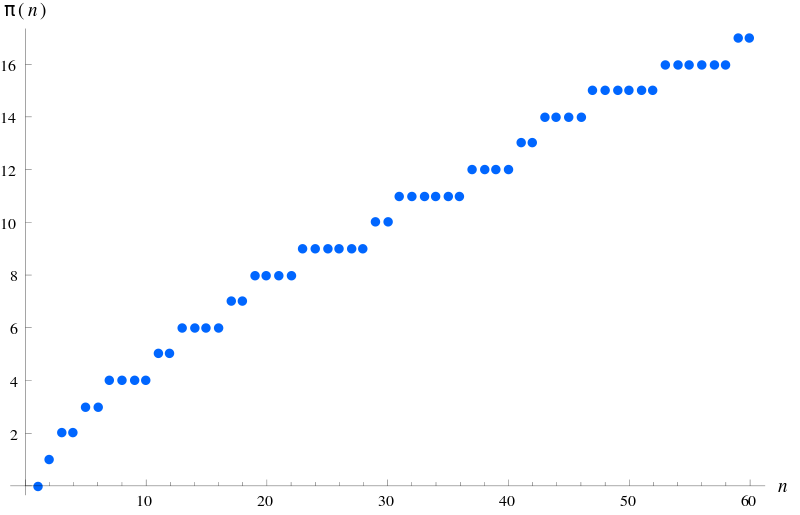
\includegraphics[width=0.6\textwidth]{prime.png}
  \end{center}
   \vspace{-10pt}
\end{wrapfigure}
\hspace{20}
Теперь построим график, используя эти значения. По оси OY будут лежать значения количества простых чисел, а по оси OX - целые числа, для которых мы ищем простые числа. Получаем соответствующий график функции распределения простых чисел



\hspace{90}$\pi(x)$


\hspace{20}Кстати, на самом деле она никак не связана с числом $\pi$.


\hspace{20}То есть функция распределения простых чисел - это функция, равная числу простых чисел, меньших либо равных действительному числу $x$. \\



\hspace{20} Как видите, это не совсем разнобой, но близко к тому. Если рассмотреть эту функцию дальше, то сходу никакой закономерности мы не увидим. И, конечно же, люди начали пытаться эту закономерность найти, чтобы прогнозировать, где искать эти самые простые числа. И один из способов их найти - это использовать дзета-функцию, которую как раз и ввел Риман. На самом деле определение не такое уж и \textbf{страшное}:
\newline 
\centerline{$\zeta(s)=\Sum_{n=1}^{\infty}\dfrac{1}{n^s} = \dfrac{1}{1^s}+\dfrac{1}{2^s}+\dfrac{1}{3^s}+\dfrac{1}{4^s}+....$}



\hspace{20}
\newline \hspace{20}
\begin{wrapfigure}{l}{0.4\textwidth}
 \vspace{-40pt}
  \begin{center}
    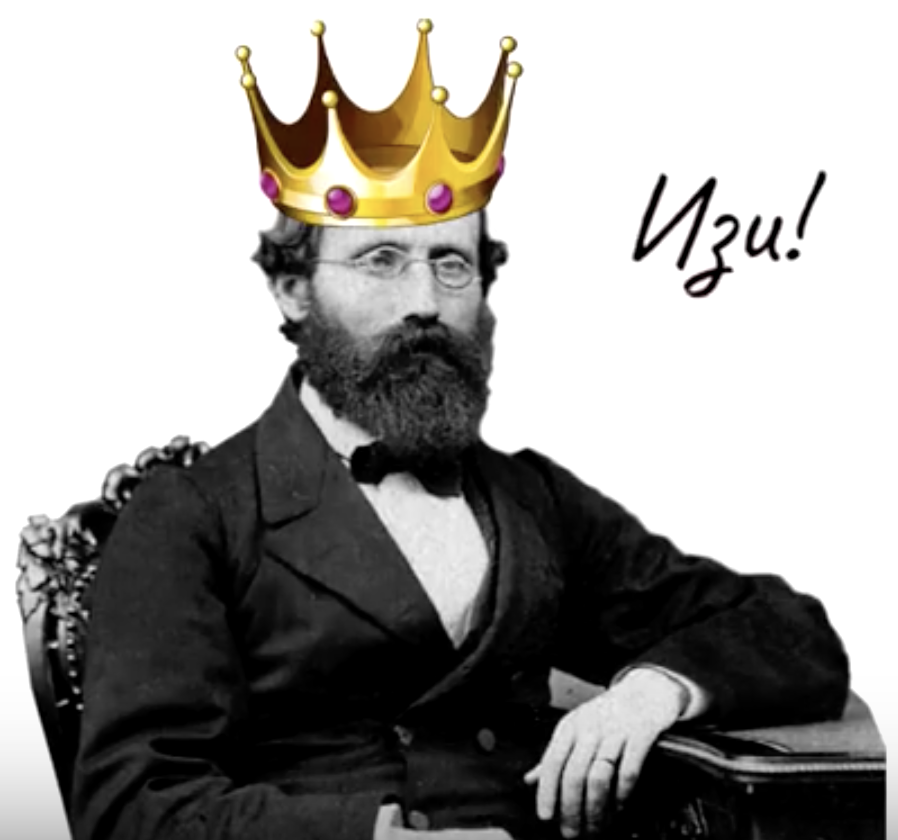
\includegraphics[width=0.3\textwidth]{easy.png}
  \end{center}
   \vspace{-80pt}
\end{wrapfigure}
\hspace{20}Все \textbf{очень легко и понятно}, по крайней мере, было таковым для Римана. Мы бы смогли увидеть нули дзета-функции, если бы построили её график. Пусть по оси OX лежат значения s, которые изменяются от 0 до $+\infty $, а по оси OY $ - $ значения, в которых данный ряд сходится, то есть, грубо говоря, чему равняется сумма данного ряда при определенных значениях s.

\newline \hspace{20}
\begin{wrapfigure}{r}{0.5\textwidth}
 \vspace{-40pt}
  \begin{center}
    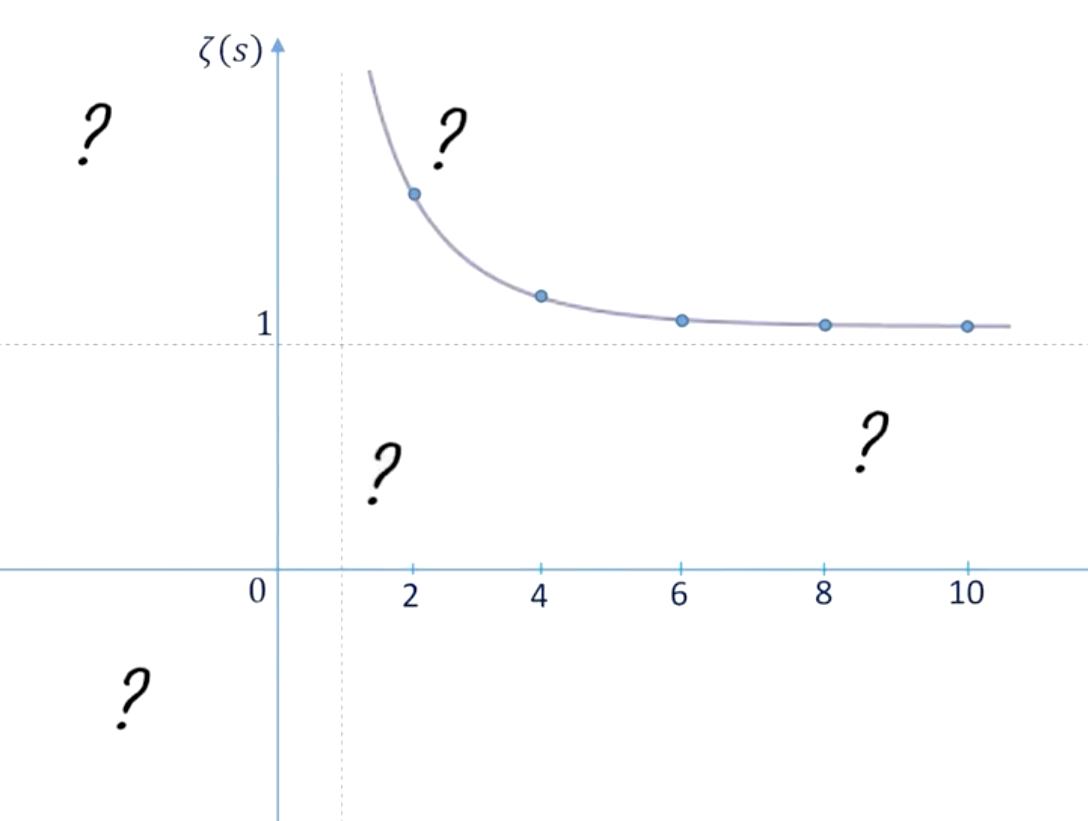
\includegraphics[width=0.4\textwidth]{zeta.png}
  \end{center}
   \vspace{-60pt}
\end{wrapfigure}
\hspace{20}
Очевидно, что данный ряд сходится для всех $s>1$, поэтому дзета-функция от единички не определена.



\hspace{20}Одно только непонятно, а где же нули дзета-функции? А еще действительная часть равна $\dfrac{1}{2}$....
Ведь если мы возьмем аргументом дзета-функции $\dfrac{1}{2}$, то получим расходимость и бесконечность. Ага! Давайте посмотрим, что предлагает нам наш \textbf{верный друг} Wolfram. Введем какое-нибудь отрицательное число:


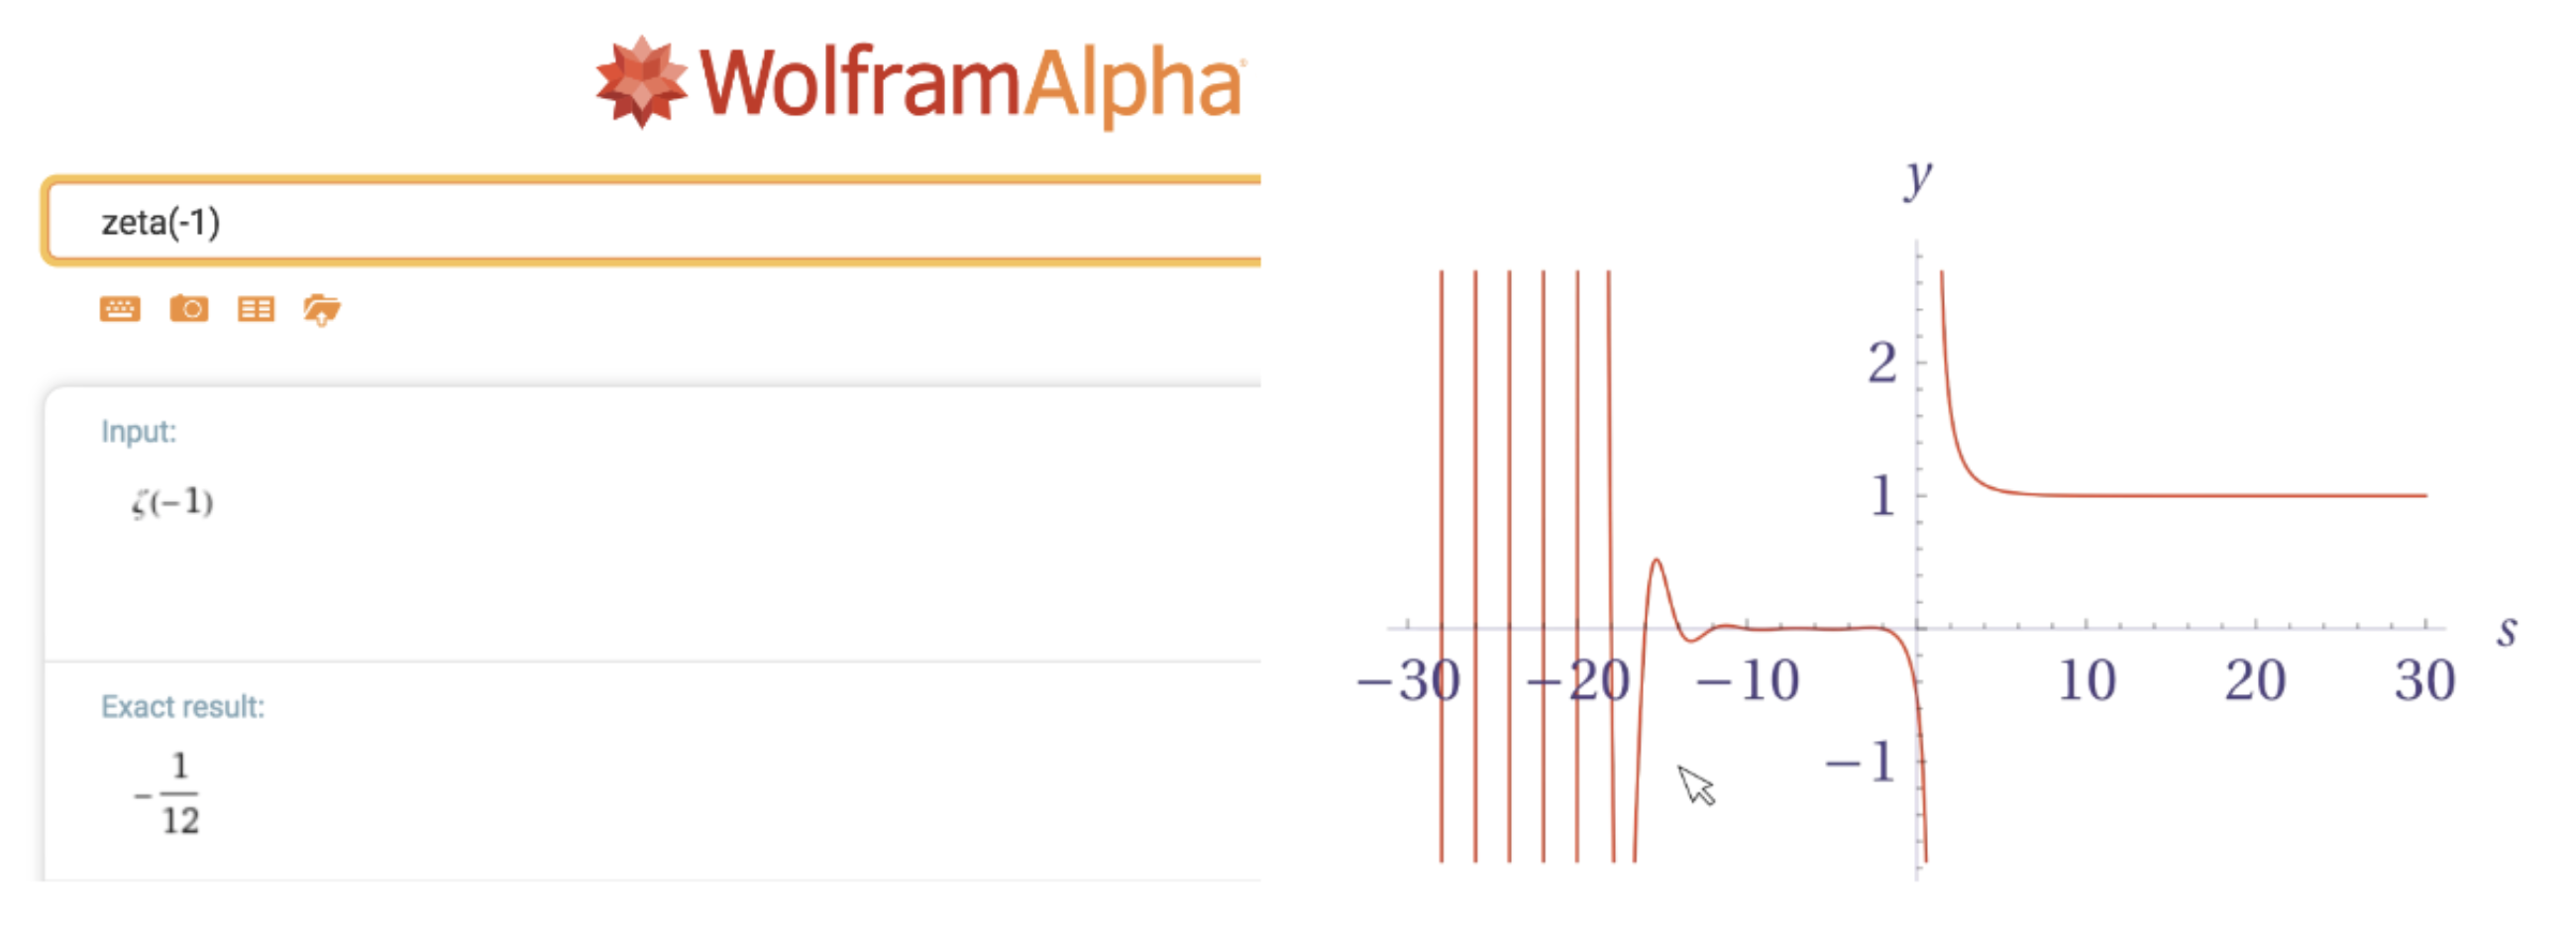
\includegraphics[width=\textwidth]{wolfram.png}




\hspace{20}Получили значение \textbf{$-\dfrac{1}{12}$}! Да и \textbf{вообще} у Вольфрама дзета определена для любых аргументов, кроме единички. Притом и нули достигаются в четных отрицательных значениях. Мда.... приехали!
И, казалось бы, вот они! Нули дзета-функции. \textbf{Но это вам не задачи на модуле решать}: тут не все так просто:) Все эти нули тривиальные, а нам интересны нетривиальные нули. 

\hspace{20}Оказывается, у некоторых функций есть \textbf{аналитическое продолжение}. Речь идет о функциях, которые дифференцируются сколько угодно раз, в ряд Тейлора раскладываются, помните такие? Они имеют продолжение в виде некоторой другой функции, кстати говоря, ЕДИНСТВЕННОЙ. То есть если мы знаем значение функции для некоторого множества комплексных чисел, мы автоматически знаем его для всех комплексных чисел, что \textbf{поражает рассудок наповал}. 

\hspace{20}И, в частности, нашу родную дзета-функцию для действительного аргумента, раз уж она подходит под все условия, можно расширить на всю комплексную плоскость по принципу аналитического продолжения. И Риман с этим справился на ура! 
Но прежде чем объяснить как именно он это сделал, давайте порассуждаем вот над чем: получается, что сумма натуральных чисел равна $-\dfrac{1}{12}$? Посмотрите сами:
\newline 
\centerline{$\zeta(-1)=-\dfrac{1}{12}=\dfrac{1}{1^{-1}}+\dfrac{1}{2^{-1}}+\dfrac{1}{3^{-1}}+\dfrac{1}{4^{-1}}+....= 1+2+3+4+5+6...$ }

\newline \hspace{20}
\begin{wrapfigure}{l}{0.4\textwidth}
 \vspace{-10pt}
  \begin{center}
    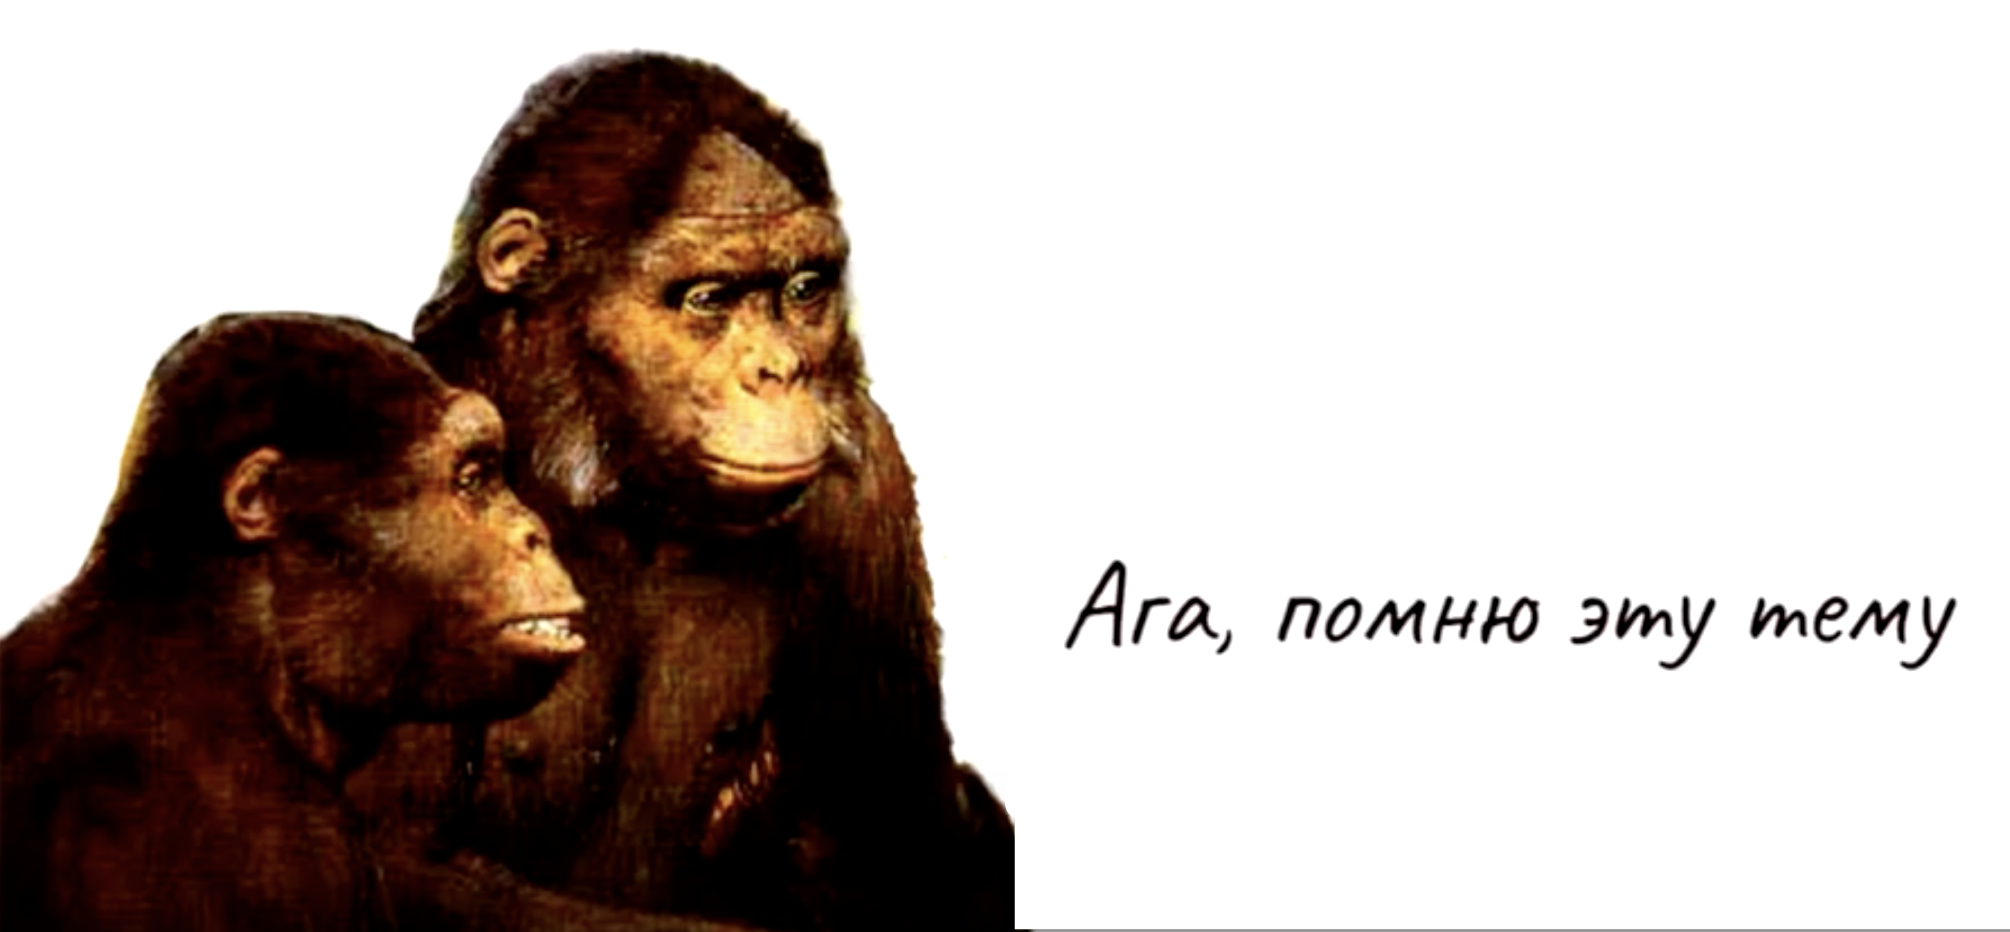
\includegraphics[width=0.4\textwidth]{primates.png}
  \end{center}
   \vspace{-25pt}
\end{wrapfigure}
\hspace{20}

\hspace{20}Не спешите сворачивать эту статью, это не очередная шутка с YouTube типа $2+2=5$! Но как же так получается, что по идее расходящаяся сумма может равняться конечному числу, при этом действительному? \textbf{Позвольте ответить вопросом на вопрос}: а разве существует квадратный корень из отрицательной единицы? Конечно, мы знаем, что сумма углов в треугольнике равна 180 градусов, параллельные прямые не пересекаются, корень из отрицательного числа не извлекается. Но чем глубже люди изучали математику, тем больше понимали, что эти правила можно нарушить. Очень много задач было решено с использованием этой самой мнимой единицы, да и вообще она помогла нам понять больше о вещественных числах.

\hspace{20}\textbf{Так вот, давайте же мы рассмотрим нашу сумму в другом контексте}, где мы, так сказать, отбросим бесконечность и оставим число, которое имеет смысл. 

\newline \hspace{20}
\begin{wrapfigure}{r}{0.35\textwidth}
 \vspace{-20pt}
  \begin{center}
    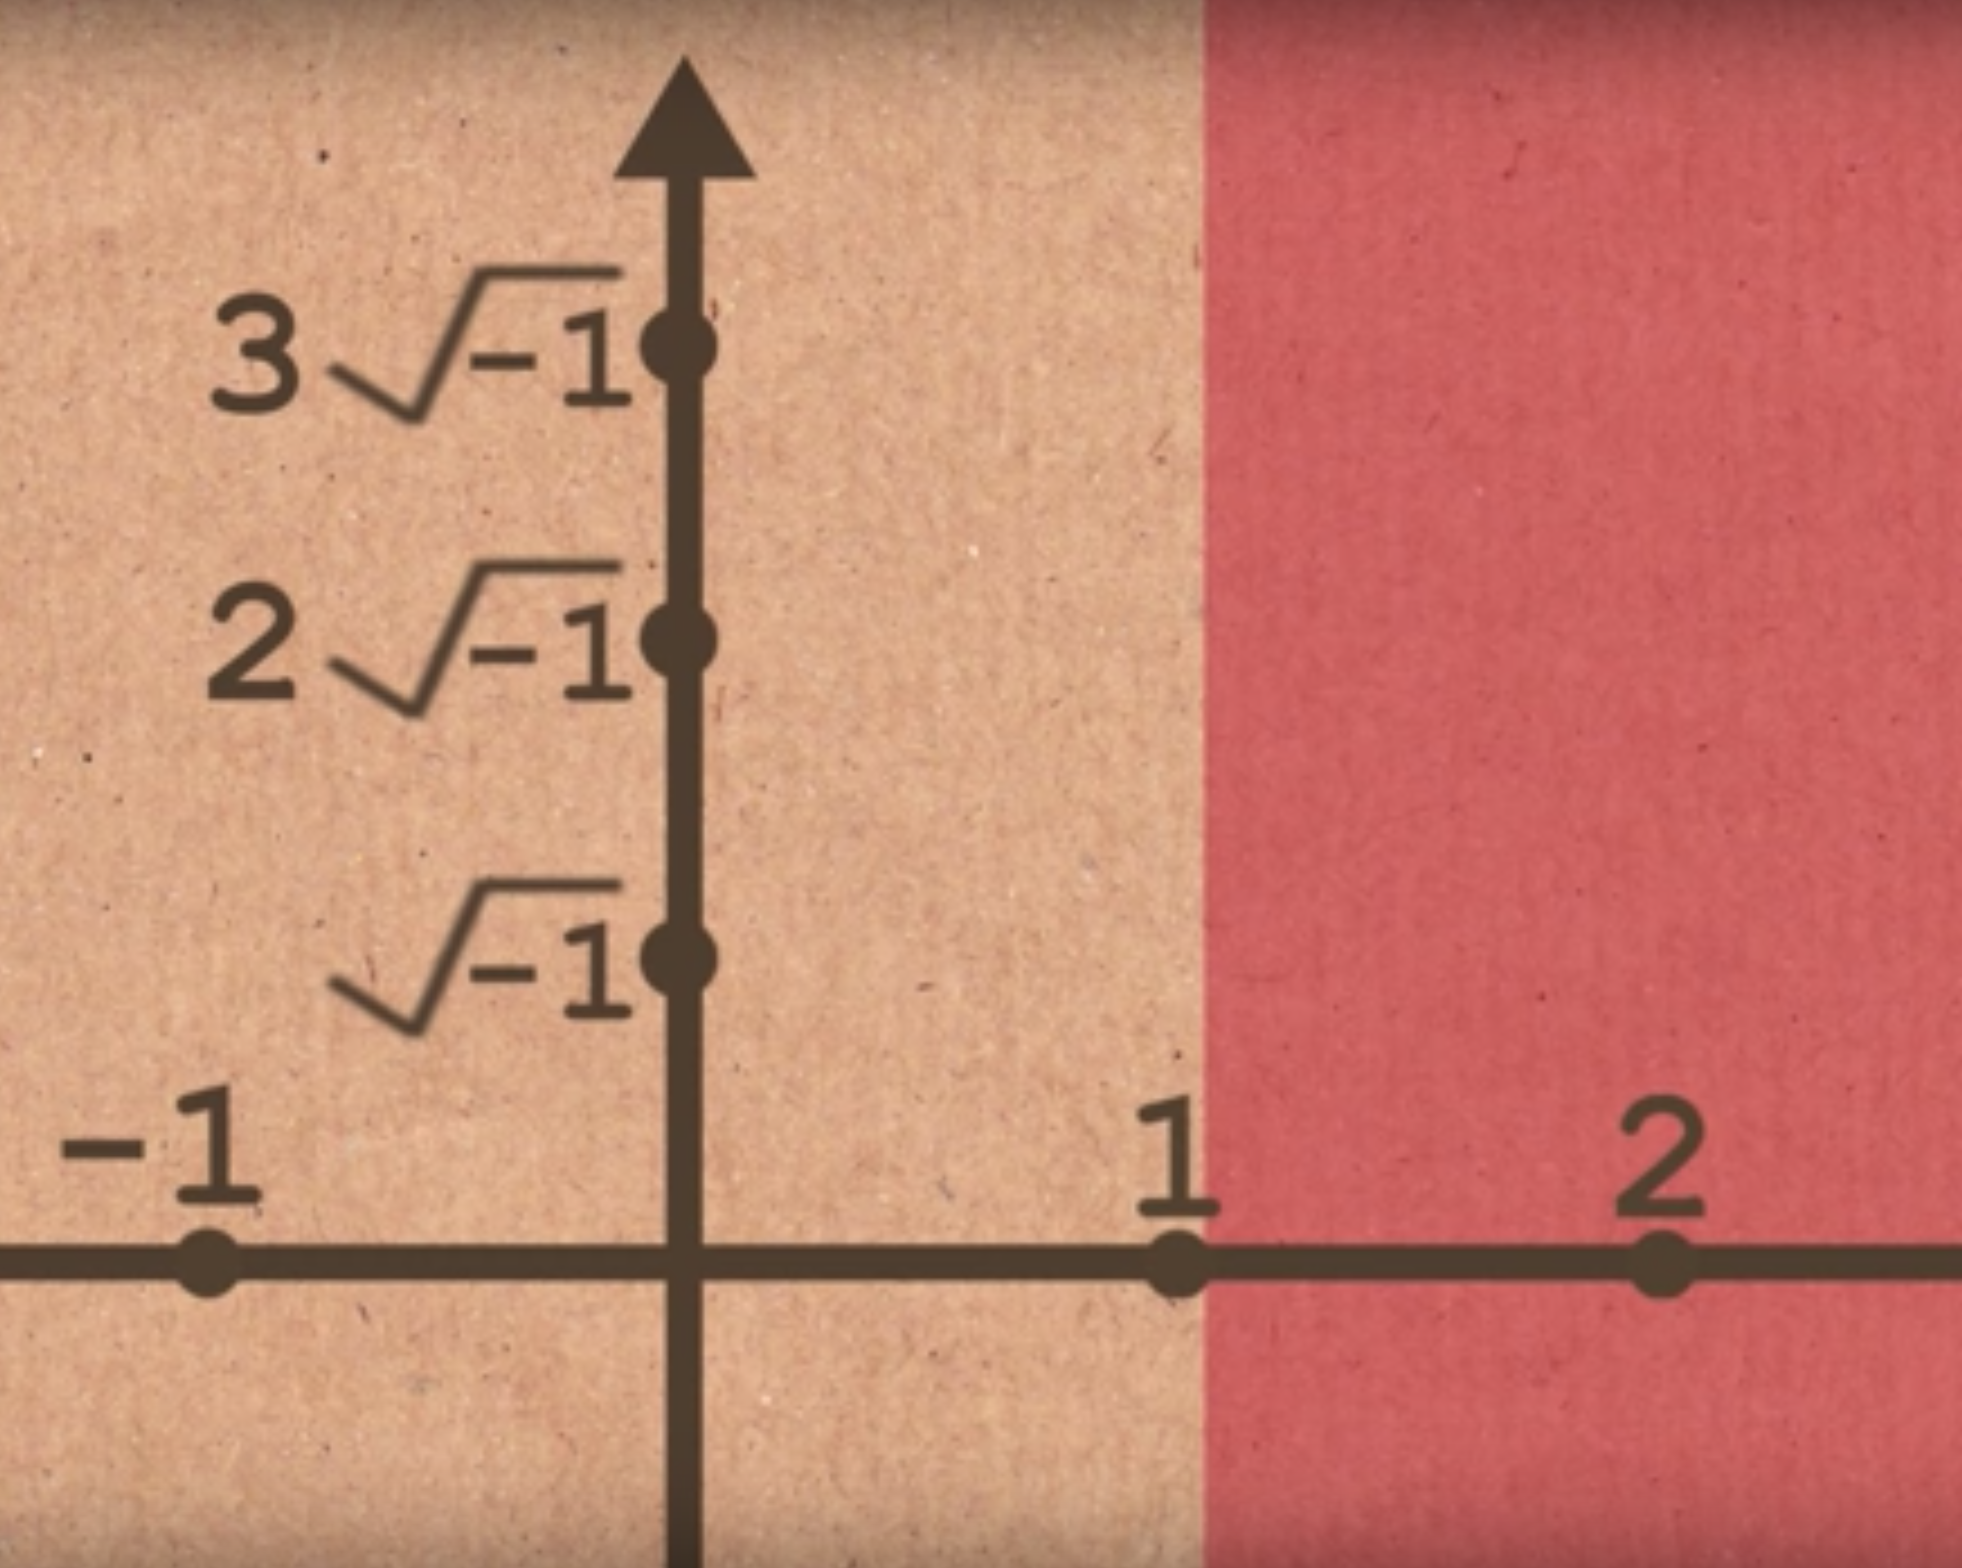
\includegraphics[width=0.3\textwidth]{red.png}
  \end{center}
   \vspace{-20pt}
\end{wrapfigure}

\hspace{20}Итак, изначально аргументом дзета-функции было любое действительное число $s>1$. Но мы можем сделать больше. Пусть теперь $s$ не действительное, а \textbf{комплексное}. То есть теперь наш ряд будет сходим не только при действительном $s$ с отрезка $(0; +\infty)$, но и при любом комплексном $s = a+bi$, расположенном в красной области (не включая прямую $s=1$, конечно же), то есть для $a>1$ и $\forall b$.
Поскольку дзета - теперь функция комплексного аргумента, то, как и утверждалось раньше, ее область определения можно расширить таким образом, чтобы в каждой точке она была определена. Риман объяснил как это сделать для всех чисел, \textbf{кроме единицы}. В этой точке существует так называемая сингулярность. Сколько не пытайся, все равно $\zeta(1) $ будет неопределенной.


\hspace{20}Риман рассмотрел следующую бесконечную сумму:\\



\centerline{$\Sum_{n=1}^{\infty} \dfrac{-1^{n+1}}{n^s}= \left(\dfrac{1}{1^s}-\dfrac{1}{2^s}+\dfrac{1}{3^s}-\dfrac{1}{4^s}+....\right)$}


\hspace{20}Далее поделил левую и правую часть на $(1-2^{1-s})$:\\



\centerline{$(1-2^{1-s})^{-1}\Sum_{n=1}^{\infty} \dfrac{-1^{n+1}}{n^s}=(1-2^{1-s})^{-1} \left(\dfrac{1}{1^s}-\dfrac{1}{2^s}+\dfrac{1}{3^s}-\dfrac{1}{4^s}+....\right)$ }

\newline \hspace{20}
\begin{wrapfigure}{r}{0.35\textwidth}
 \vspace{-20pt}
  \begin{center}
    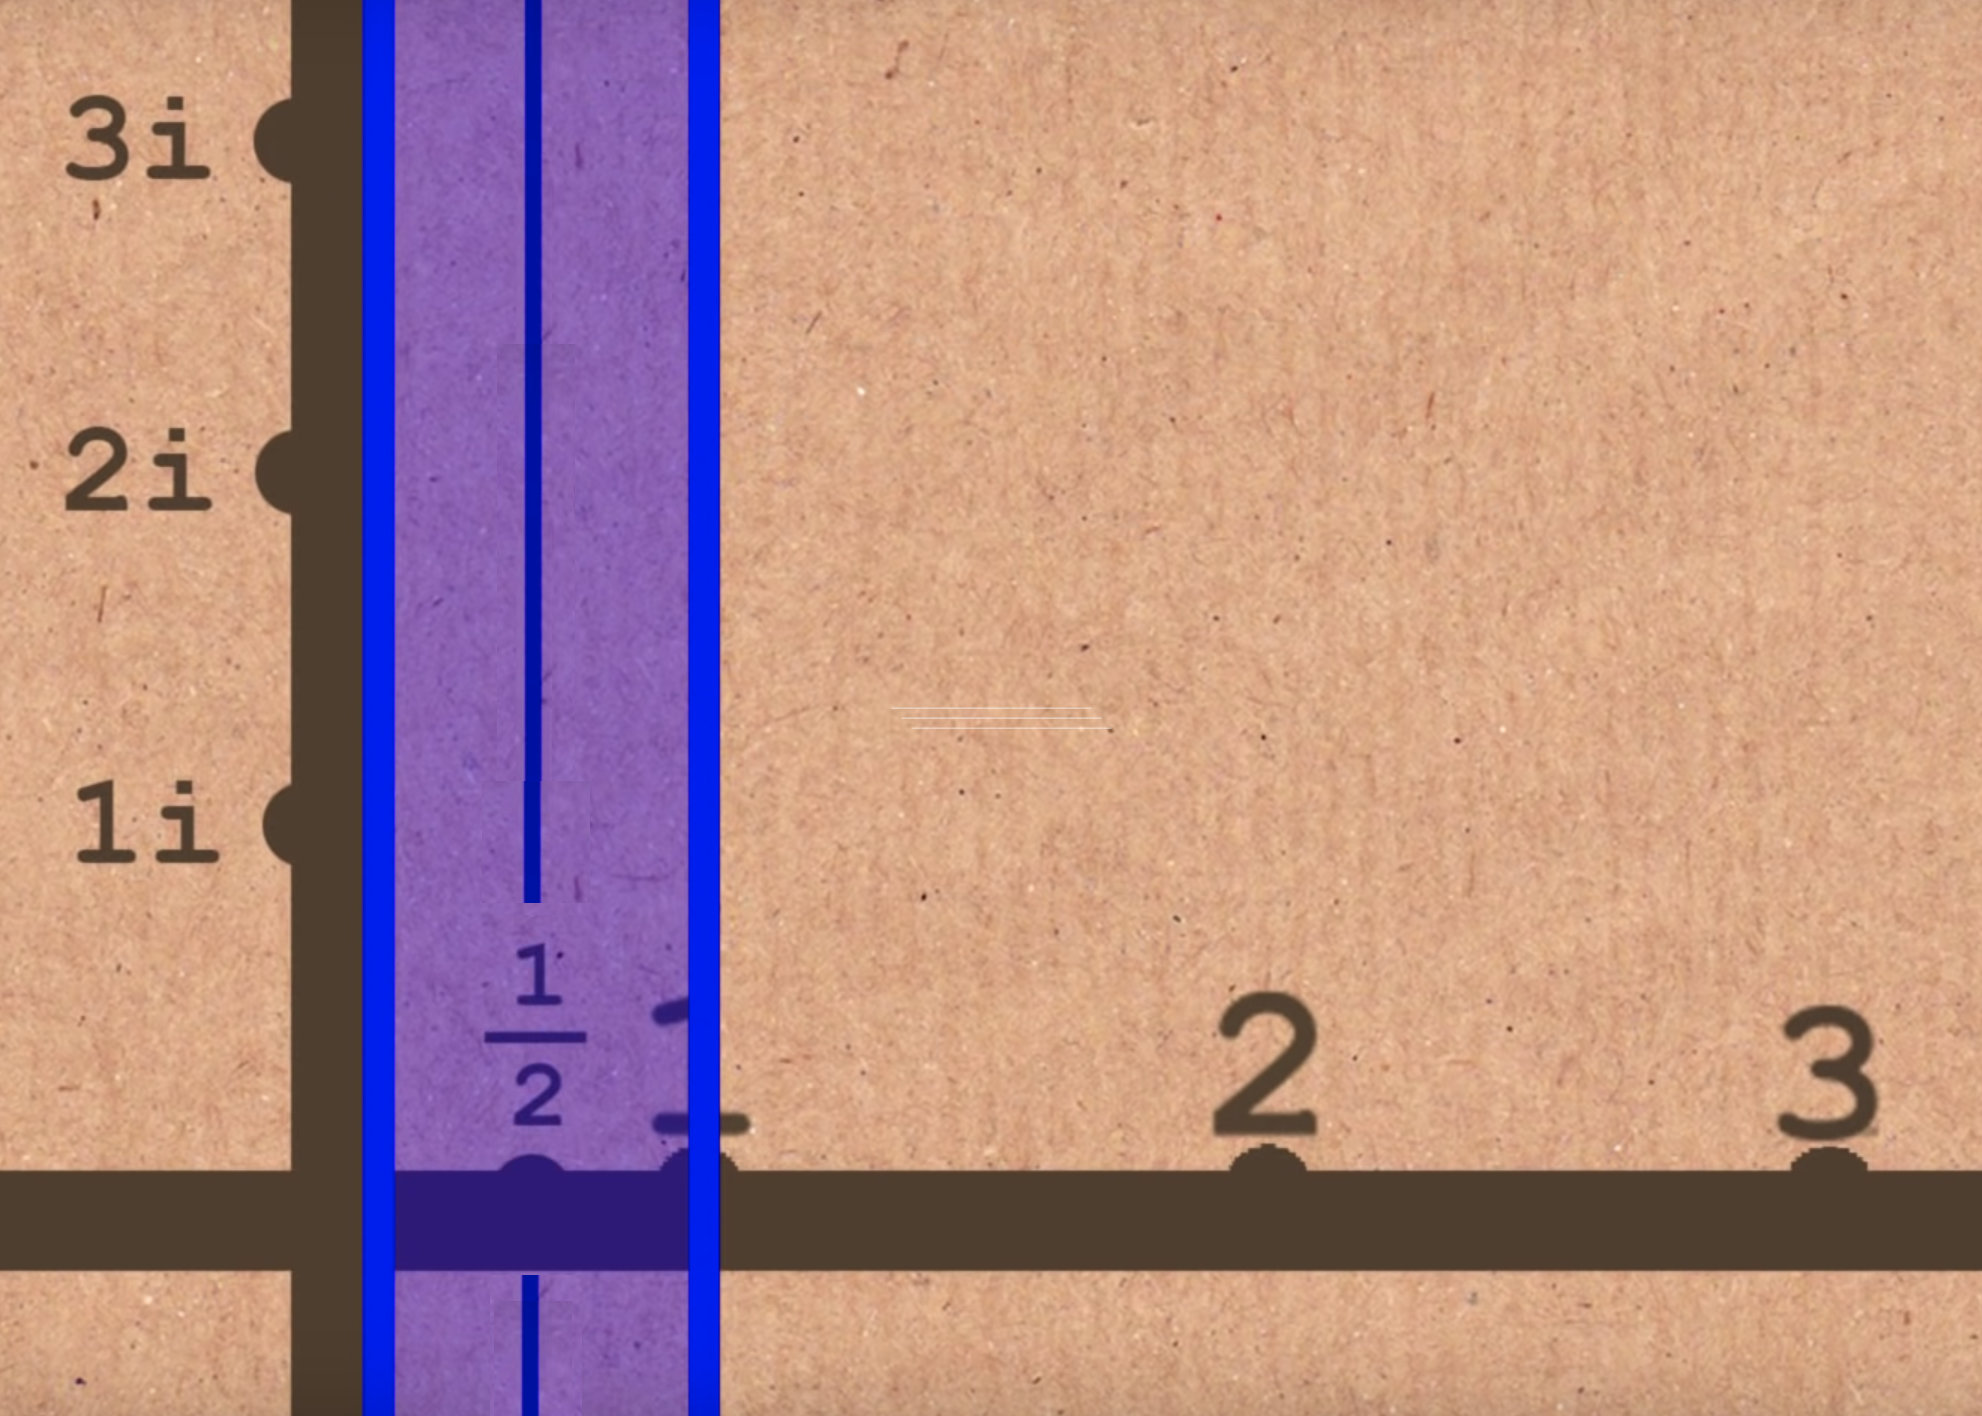
\includegraphics[width=0.3\textwidth]{blue.png}
  \end{center}
   \vspace{-60pt}
\end{wrapfigure}
\hspace{20} Риману удалось показать, что эта новая функция,\\

$f(x) = (1-2^{1-s})^{-1}\Sum_{n=1}^{\infty} \dfrac{-1^{n+1}}{n^s}$, определена для всех $s=a+bi$, где $Re(s) > 0\; (a>0)$.  И она равна нашей изначальной функции $\zeta(s)$ при $Re(s) >1$. Хорошо, с положительными значениями $s$ мы разобрались. А что будет при отрицательных? Здесь уже совсем другой подход. Риман рассмотрел часть функции, где $Re(s) \in (0; \:1) \;- $ наша синяя область. В этом промежутке выполняется равенство:



\hspace{90}$\zeta (s)=2^{s}\pi ^{s-1}\sin \left({\dfrac{\pi s}{2}}\right)\Gamma (1-s)\zeta (1-s)$\\



\hspace{20} Как можно увидеть в формуле, значение функции в точках $(s)$ и $(1-s)$ как бы отражены, причем относительно нашей старой знакомой прямой $s=\dfrac{1}{2}$, и умножены на этот страшный коэффициент с числом $\pi$, синусом и гамма-функцией. \textbf{Ну наконец-то она нам пригодилась в жизни!} Так вот, мы можем с помощью этой формулы отразить все наши положительные значения на отрицательные, говоря простым языком. И, таким образом, наша функция будет определена. Давайте проверим, что там Wolfram говорил? Какое там значение функции в точке $(-1)$?\\


\hspace{20}$\zeta(-1) = 2^{-1}\pi ^{-1-1}\sin \left({\dfrac{\pi (-1)}{2}}\right)\Gamma (1-(-1))\zeta (1-(-1))= -\dfrac{1}{2\pi^2} \zeta(2) = \\

\hspace{20}=\left |$а значение в точке $s=2$ мы знаем $|\right| =-\dfrac{1}{2\pi^2} \dfrac{\pi^2}{6} =- \dfrac{1}{12}$. Ура! 
Все гениальное \sout{просто}!\\

\hspace{20}Таким образом, мы как бы упорядочиваем нашу бесконечную сумму и присваиваем ей число. Конечно, теперь нельзя просто полагать, что СУММА натуральных чисел равна $-\dfrac{1}{12}$. Последнее число уже не просто сумма, оно было получено путем сложной процедуры расширения функции комплексного аргумента за пределы первоначальной области определения. И под "дзета"$\:$  уже понимаем аналитически продолженную функцию. 





\hspace{20}А теперь \textbf{вопрос на миллион}: для каких $s \;\; \zeta(s) = 0$?
Тривиальные нули видны с формулы невооруженным глазом: парные отрицательные. Посмотрите повнимательнее на синус:\\
\centerline{$\left(\sin{\dfrac{\pi s }{2}} \right)=0 \iff s = -2k, \:k \in \mathbf{Z}$.}

\hspace{20}\textbf{А где остальные нули?} Очевидно, что они будут находиться только в синей области - это все комплексные числа $s = a + bi$, у которых $a \in (0; 1)$.
Внутри этой области проведена линия $s=\dfrac{1}{2}$. И как раз-таки на этой прямой лежат нетривиальные нули дзета функции, по гипотезе Римана, то есть $s = \dfrac{1}{2}+bi$. А если найдётся хоть одно число, лежащее внутри этой области, но не на упомянутой прямой, то гипотеза будет опровергнута. 

\section{Так вот зачем все это нужно!}

\hspace{20} Наверняка у вас возник вопрос: \textbf{"A зачем вообще вначале упоминалось про простые числа?"} Дело в том, что Риман обнаружил - поведение и местонахождение нулей дзета-функции имеет прямое отношение к распределению простых чисел, а именно, функция распределения простых чисел выражается через распределение нетривиальных нулей дзета-функции.

\hspace{20}\textbf{Так а в чем же связь этой дзета-функции с простыми числами?} Вообще, есть такая очень красивая формула:


\centerline{$\zeta(s)=\Sum_{n=1}^{\infty}\dfrac{1}{n^s}={\displaystyle \prod_{p}^{} }\dfrac{1}{1-p^{-s}}$}\\
Малая буква $p$ пробегает все простые числа. Доказывать ее мы не будем - доказательство прочитаете на Википедии, оно несложное и довольно интересное.


\hspace{20}Но вот 15-летний Эйлер углядел следующее: 


\hspace{220}$\Lim_{x \to \infty} \dfrac{\pi(x)}{x/lnx} = 1$ \\

\hspace{20}Данное равенство называется \textbf{теоремой о распределении простых чисел}. \\

\hspace{20}Как пример рассмотрим значение в точке 100: $\pi(100)\approx \dfrac{100}{ln100}$\approx 21,71$. Это вполне близкий к истине результат, который, как мы помним, равен 25. 

\hspace{20}Позже Гауссу удалось вывести более точную формулу:


\hspace{220}$\pi(x) \approx \Int_2^x  \dfrac{\mathrm{d}t}{lnt}$


\hspace{20}Но и это число приближенное, а не точное. Для некоторых аргументов оно может даже существенно отличаться от настоящего на какое-то значение. \textbf{Так и есть, так и есть!} При достаточно больших аргументах ошибка составляет миллионы чисел, например, при $s=10^{25}$ результат по Гауссу отличался бы от настоящего значение функции $\pi(x)$ на 55160980939! Конечно же, это число мизерно мало по сравнению с $10^{25}$, но все же, если бы мы захотели составить список простых чисел меньше либо равных числу $10^{25}$, были бы утеряны 55160980939 простых чисел. 
%%%%%%%%%%%%%%%%%%%%%%%%%%%%%%%%%%%%%%%%%%%%%%%%%



\hspace{20}\textbf{А теперь внимание!} Сейчас вы увидите, как именно нули дзета-функции связаны с функцией распределения простых чисел. 
Если гипотеза Римана окажется верна, мы получим точное,  \textbf{понимаете?}, ТОЧНОЕ значение дзета-функции для заданного числа. И вот чему оно будет равно:\\


\hspace{200}${\pi (x)=R (x)-\Sum _{\rho }R(x^{\rho })$\\


где, R(x)=\Sum _{n=1}^{\infty }{\dfrac {\mu (n)}{n}}li (x^{1/n})$

\hspace{24}$li(x)=\Int _{0}^{x}{\dfrac {dt}{\ln t}} \,- $ интегральный логарифм, \\

\hspace{24}$\mu (n)=\Sum_{\stackrel {1\leq k\leq n}{\gcd(k,\,n)=1}}e^{2\pi i{\frac {k}{n}}} \, - $ функция Мёбиуса. \\ 

\hspace{24}А вот $\rho  - $ это как раз комплексные \textbf{нули дзета-функции Римана}, которые, по гипотезе, все лежат на прямой $Re(s) = \dfrac{1}{2}$.


\hspace{20}Конечно же, осмыслить написанное трудно, ибо нам не хватает знаний. Так что давайте просто поверим Риману и будем  \textbf{восхищаться} тем, что такую связь между простыми числами и нулями дзета-функции вообще удалось увидеть! В этом и есть красота математики и за это я ее люблю: посредством сложных математических вычислений, нарушением правил и придумыванием новых функций мы приходим к чему-то совершенно простому и понятному. И это абсолютно невероятно! Ведь сразу и неясно, что такая простая вещь, как простые числа (думаю, тавтология здесь только уместна) может быть связана с "темным лесом" \; комплексных чисел, аналитическим продолжением и т.д. Удивительно, что эти две вещи так тесно существуют! 

\hspace{20}\textbf{Вот вам и вывод}: если вдруг мы научимся понимать, как устроена дзета-функция, то через это начнем понимать и то, как устроена функция $\pi(x)$. Например, сколько простых чисел до триллиона? Сразу сложно сказать, но есть формула, которая дает точный ответ. \textbf{Именно поэтому} гипотеза Римана настолько важна.

\section{А что же происходит сейчас?}
\newline \hspace{20}
\begin{wrapfigure}{l}{0.5\textwidth}
 \vspace{-20pt}
  \begin{center}
    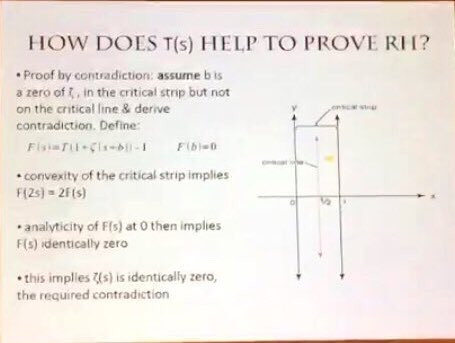
\includegraphics[width=0.4\textwidth]{slide.jpg}
  \end{center}
   \vspace{-20pt}
\end{wrapfigure}
\hspace{20}Атья собрал пресс-конференцию и выступил со своим докладом. Он не столько заинтриговал, сколько напряг слушателей, потому что доказательству был посвящен всего лишь один слайд. И чуть более чем десятком строчек он утверждает, что решил одну из самых таинственных загадок математики. Ведущие умы мира пытаются подтвердить или опровергнуть это доказательство, а мы с вами затаились в ожидании. Хотя не теряйте время зря и 
сами попытайтесь доказать гипотезу Римана - чем не занятие на выходные:) \textbf{Только не вздумайте списывать у Атьи!}\\
  

\newline



\vspace{45}

\newline


\hspace{345} \textit{\textbf{Логвина Ангелина}}




\hspace{345} \textit{студентка КНУ им. Т.Г. Шевченка,}




\hspace{345} \textit{факультет компьютерных наук и}





\hspace{345} \textit{кибернетики,}



\hspace{345} \textit{прикладная математика}



\end{document}
